% !TEX program = pdflatex
\documentclass[11pt,a4paper]{article}

\usepackage[margin=1.8cm]{geometry}
\usepackage{amsmath,amssymb}
\usepackage{array,booktabs}
\usepackage{enumitem}
\usepackage{tikz}
\usepackage{pgfplots}
\usepackage{fancyhdr}
\usepackage{tabularx}
\usepackage{multicol}
\usepackage{graphicx}
\usepackage{xcolor}
\usepackage{siunitx}

\pgfplotsset{compat=1.18}
\usetikzlibrary{angles,quotes,calc,arrows.meta}

\pagestyle{fancy}
\fancyhf{}
\lhead{DJA Ostbevern 2026}
\rhead{Mathematics of Acoustics}
\cfoot{\thepage}
\setlength{\headheight}{14pt}

\setlist[enumerate]{itemsep=0.35em}
\setlength{\parindent}{0pt}
\setlength{\parskip}{0.5em}

\newcommand{\answerline}[1][4cm]{\rule{#1}{0.4pt}}
\newcommand{\blank}[1]{\underline{\hspace{#1}}}

\begin{document}

% ============================================================
% PAGE 1
% ============================================================

\section*{Exercise 1}
For each triangle, mark the hypotenuse with $H$, the side opposite the marked
angle with $O$, and the adjacent side with $A$.
Calculate $\sin$ and $\cos$ of the marked angles. What do you observe
regarding similar triangles?

\begin{center}
\begin{tikzpicture}[scale=0.8]
  % triangle 1
  \draw (0,0) -- (3,0) -- (3,2) -- cycle;
  \draw (2.7,0) rectangle +(0.3,0.3);
  \draw (0.55,0) arc (0:34:0.55);
  \node at (0.72,0.18) {$\alpha$};

  % triangle 2
  \begin{scope}[xshift=5cm]
    \draw (0,0) -- (4,0) -- (4,2.7) -- cycle;
    \draw (3.7,0) rectangle +(0.3,0.3);
    \draw (0.8,0) arc (0:34:0.8);
    \node at (0.95,0.22) {$\alpha$};
  \end{scope}

  % triangle 3
  \begin{scope}[yshift=-7cm]
    \draw (0,0) -- (2.5,0) -- (2.5,4) -- cycle;
    \draw (2.2,0) rectangle +(0.3,0.3);
    \draw (0.5,0) arc (0:58:0.5);
    \node at (0.68,0.30) {$\beta$};
  \end{scope}

  % triangle 4
  \begin{scope}[xshift=5cm,yshift=-7cm]
    \draw (0,0) -- (3,0) -- (3,5) -- cycle;
    \draw (2.7,0) rectangle +(0.3,0.3);
    \draw (0.55,0) arc (0:59:0.55);
    \node at (0.72,0.33) {$\beta$};
  \end{scope}
\end{tikzpicture}
\end{center}

\section*{Exercise 2}
A right triangle has a hypotenuse of \SI{10}{cm}. The side opposite the
angle $\alpha$ has length \SI{6}{cm}.

\begin{enumerate}%[label=\alph*)]%
    \item Use Pythagoras' theorem to calculate the adjacent side.
    \item Calculate $\sin(\alpha)$ and $\cos(\alpha)$.
    \item Calculate $\sin^2(\alpha)+\cos^2(\alpha)$.
\end{enumerate}

Do you think the result is just a coincidence?

\begin{center}
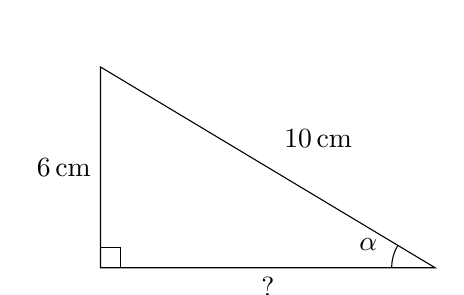
\begin{tikzpicture}[scale=0.85]
  \draw (0,0) -- (5,0) -- (0,3) -- cycle;
  \draw (0,0) rectangle +(0.3,0.3);
  \node[left] at (0,1.5) {\SI{6}{cm}};
  \node[above right] at (2.6,1.65) {\SI{10}{cm}};
  \node[below] at (2.5,0) {$?$};
  \draw (4.35,0) arc (180:149:0.65);
  \node at (4.0,0.35) {$\alpha$};
\end{tikzpicture}
\end{center}

\section*{Exercise 3}
A ladder of length \SI{5}{m} leans against a wall. The angle between the
ladder and the ground is $60^\circ$.

How can you calculate the height $h$? Write down an equation for $h$.

\begin{center}
\begin{tikzpicture}[scale=0.8]
  \draw (0.2,0) -- (4.5,0);
  \draw (3.5,0) -- (3.5,4.33);
  \draw (0.2,0) -- (3.5,4.33);
  \draw (0.2,0) -- (3.5,0);
  \node[above left] at (1.7,2.3) {\SI{5}{m}};
  \node[left] at (3.5,2.2) {$h$};
  \node at (1.1,0.28) {$60^\circ$};
  \draw (0.7,0) arc (0:52:0.5);
\end{tikzpicture}
\end{center}

\newpage

% ============================================================
% PAGE 2
% ============================================================

\section*{Exercise 4}
Complete the table. Remember that $360^\circ=2\pi$.

\begin{center}
\renewcommand{\arraystretch}{1.5}
\begin{tabular}{c|c||c|c}
\toprule
Degrees & Radians & Degrees & Radians\\
\midrule
$0^\circ$   & & $180^\circ$ & \\
$30^\circ$  & & $270^\circ$ & \\
$45^\circ$  & & $360^\circ$ & \\
$60^\circ$  & & & $\dfrac{3\pi}{2}$\\
$90^\circ$  & & & $\dfrac{\pi}{4}$\\
\bottomrule
\end{tabular}
\end{center}

\section*{Exercise 5}
The radius of the unit circle is $1$. For an angle $\alpha$, the point on the
circle has coordinates
\[
(\cos\alpha,\sin\alpha).
\]

Label the points $A$--$D$ with their coordinates and complete the table.

\begin{center}
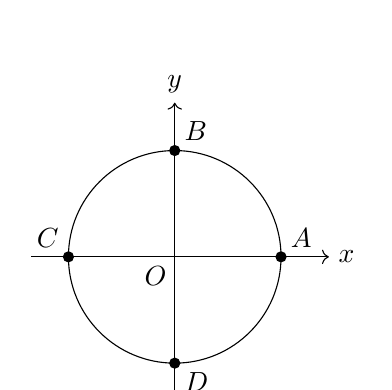
\begin{tikzpicture}[scale=1.35]
  \draw[->] (-1.35,0) -- (1.45,0) node[right] {$x$};
  \draw[->] (0,-1.35) -- (0,1.45) node[above] {$y$};
  \draw (0,0) circle (1);
  \fill (1,0) circle (1.5pt) node[above right] {$A$};
  \fill (0,1) circle (1.5pt) node[above right] {$B$};
  \fill (-1,0) circle (1.5pt) node[above left] {$C$};
  \fill (0,-1) circle (1.5pt) node[below right] {$D$};
  \node at (-0.18,-0.18) {$O$};
\end{tikzpicture}
\hspace{1.5cm}
\begin{tabular}{c|c|c}
\toprule
Angle & $\cos\alpha$ & $\sin\alpha$\\
\midrule
$0$ & & \\
$\dfrac{\pi}{2}$ & & \\
$\pi$ & & \\
$\dfrac{3\pi}{2}$ & & \\
$2\pi$ & & \\
\bottomrule
\end{tabular}
\end{center}

\newpage

% ============================================================
% PAGE 3 -- EXERCISE 13
% ============================================================

\section*{Exercise 13: What does the factor in front do?}
Compare the three graphs.

\begin{center}
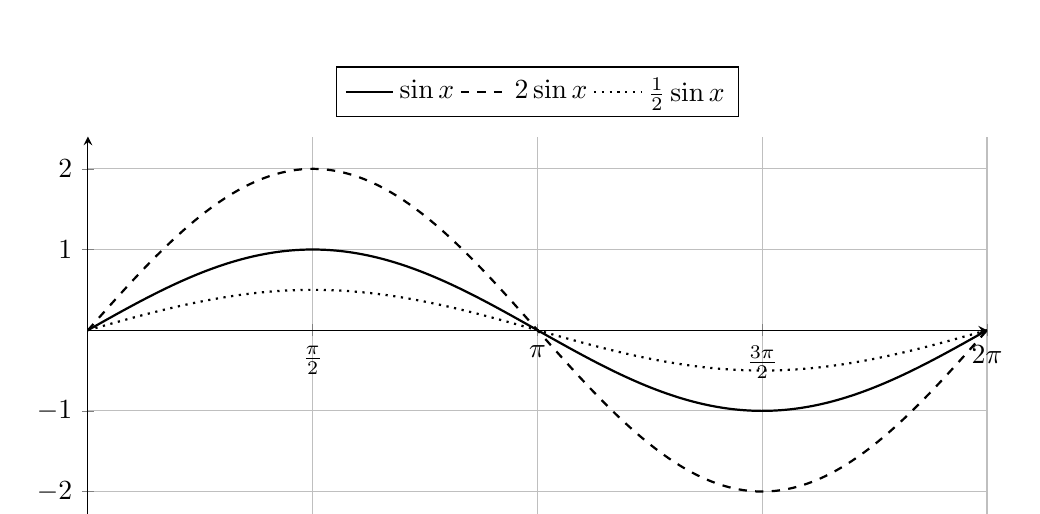
\begin{tikzpicture}
\begin{axis}[
    width=13cm,height=6.5cm,
    axis lines=middle,
    xmin=0,xmax=2*pi,
    ymin=-2.4,ymax=2.4,
    xtick={0,pi/2,pi,3*pi/2,2*pi},
    xticklabels={$0$,$\frac{\pi}{2}$,$\pi$,$\frac{3\pi}{2}$,$2\pi$},
    ytick={-2,-1,1,2},
    samples=200,
    domain=0:2*pi,
    legend style={at={(0.5,1.05)},anchor=south,legend columns=3},
    grid=major
]
\addplot[thick] {sin(deg(x))};
\addlegendentry{$\sin x$}
\addplot[thick,dashed] {2*sin(deg(x))};
\addlegendentry{$2\sin x$}
\addplot[thick,dotted] {0.5*sin(deg(x))};
\addlegendentry{$\frac12\sin x$}
\end{axis}
\end{tikzpicture}
\end{center}

\begin{enumerate}[label=\alph*)]
\item Complete the table.

\begin{center}
\renewcommand{\arraystretch}{1.5}
\begin{tabular}{c|c|c}
\toprule
Function & Amplitude & Period\\
\midrule
$\sin x$ & & \\
$2\sin x$ & & \\
$\frac12\sin x$ & & \\
\bottomrule
\end{tabular}
\end{center}

\item What changes when the factor in front of the sine changes?
\end{enumerate}

\newpage

% ============================================================
% PAGE 4 -- EXERCISES 14/15
% ============================================================

\section*{Part D continued: Frequency and Phase Shift}

\subsection*{Exercise 14: What does the factor inside do?}
Compare $y=\sin(x)$ and $y=\sin(2x)$.

\begin{center}
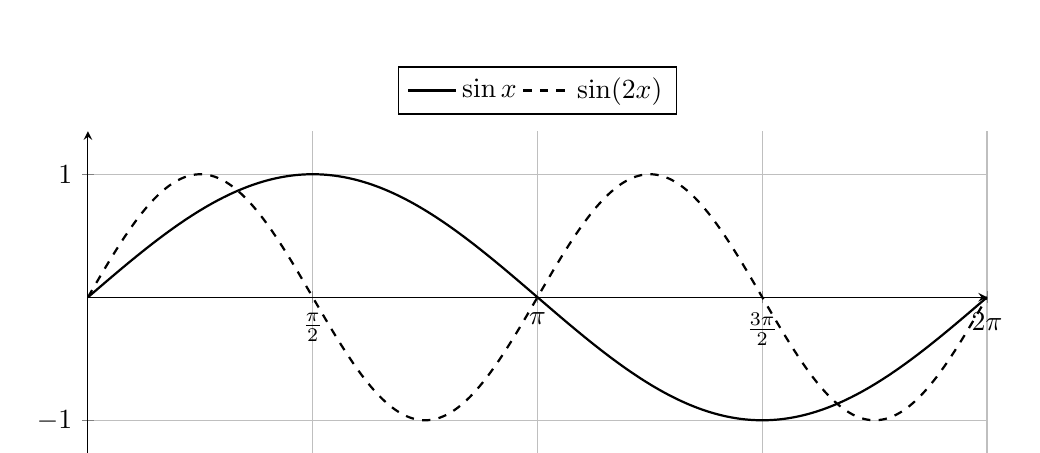
\begin{tikzpicture}
\begin{axis}[
    width=13cm,height=5.8cm,
    axis lines=middle,
    xmin=0,xmax=2*pi,
    ymin=-1.35,ymax=1.35,
    xtick={0,pi/2,pi,3*pi/2,2*pi},
    xticklabels={$0$,$\frac{\pi}{2}$,$\pi$,$\frac{3\pi}{2}$,$2\pi$},
    ytick={-1,1},
    samples=300,
    domain=0:2*pi,
    legend style={at={(0.5,1.05)},anchor=south,legend columns=2},
    grid=major
]
\addplot[thick] {sin(deg(x))};
\addlegendentry{$\sin x$}
\addplot[thick,dashed] {sin(deg(2*x))};
\addlegendentry{$\sin(2x)$}
\end{axis}
\end{tikzpicture}
\end{center}

\begin{enumerate}[label=\alph*)]
\item How many complete oscillations does each graph make between $0$ and $2\pi$?
\item Which graph has the shorter period? \answerline
\item Complete: The period of $\sin(2x)$ is \answerline
\item Does the amplitude change? \answerline
\end{enumerate}

\subsection*{Exercise 15: Match equations and graphs}
Match each graph A--D to one equation. Write the correct letter next to each equation.

\begin{center}
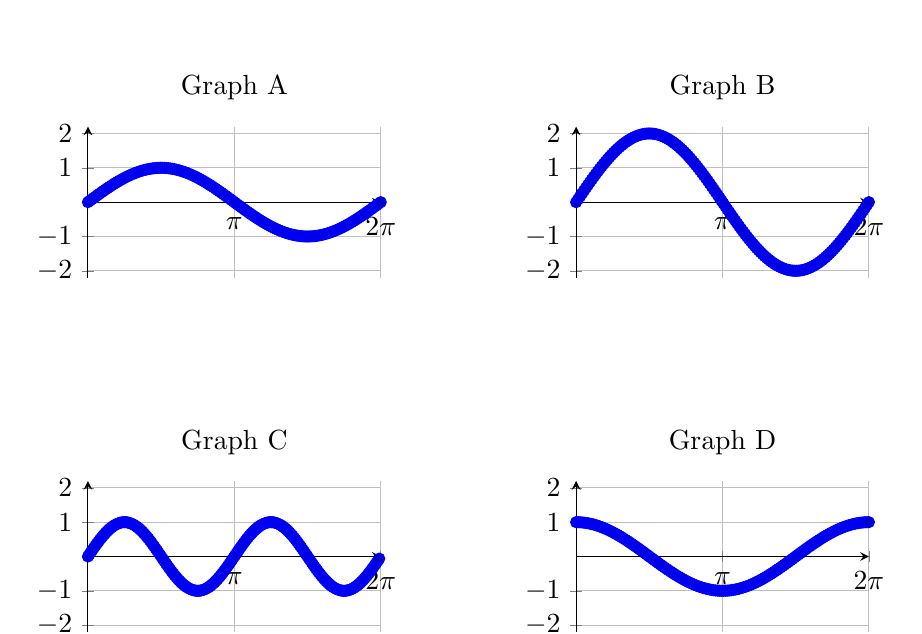
\begin{tikzpicture}
\begin{axis}[name=A,width=5.3cm,height=3.5cm,axis lines=middle,
  xmin=0,xmax=2*pi,ymin=-2.2,ymax=2.2,
  xtick={pi,2*pi},xticklabels={$ \pi$,$2\pi$},ytick={-2,-1,1,2},
  samples=150,domain=0:2*pi,grid=major,title={Graph A}]
\addplot {sin(deg(x))}; \end{axis}

\begin{axis}[name=B,xshift=6.2cm,width=5.3cm,height=3.5cm,axis lines=middle,
  xmin=0,xmax=2*pi,ymin=-2.2,ymax=2.2,
  xtick={pi,2*pi},xticklabels={$ \pi$,$2\pi$},ytick={-2,-1,1,2},
  samples=150,domain=0:2*pi,grid=major,title={Graph B}]
\addplot {2*sin(deg(x))}; \end{axis}

\begin{axis}[name=C,yshift=-4.5cm,width=5.3cm,height=3.5cm,axis lines=middle,
  xmin=0,xmax=2*pi,ymin=-2.2,ymax=2.2,
  xtick={pi,2*pi},xticklabels={$ \pi$,$2\pi$},ytick={-2,-1,1,2},
  samples=200,domain=0:2*pi,grid=major,title={Graph C}]
\addplot {sin(deg(2*x))}; \end{axis}

\begin{axis}[name=D,xshift=6.2cm,yshift=-4.5cm,width=5.3cm,height=3.5cm,axis lines=middle,
  xmin=0,xmax=2*pi,ymin=-2.2,ymax=2.2,
  xtick={pi,2*pi},xticklabels={$ \pi$,$2\pi$},ytick={-2,-1,1,2},
  samples=150,domain=0:2*pi,grid=major,title={Graph D}]
\addplot {cos(deg(x))}; \end{axis}
\end{tikzpicture}
\end{center}

\begin{multicols}{2}
\begin{itemize}[label=$\square$]
\item $y=\sin(x)$ \hfill \blank{0.6cm}
\item $y=2\sin(x)$ \hfill \blank{0.6cm}
\item $y=\sin(2x)$ \hfill \blank{0.6cm}
\item $y=\cos(x)$ \hfill \blank{0.6cm}
\end{itemize}
\end{multicols}

\newpage

% ============================================================
% PAGE 5 -- EXERCISES 16/17
% ============================================================

\section*{Part E: Sketching and Explaining}

\subsection*{Exercise 16: Sketch the graphs}
Sketch one complete period of each function. Mark the zeros, maxima, and minima.

\begin{center}
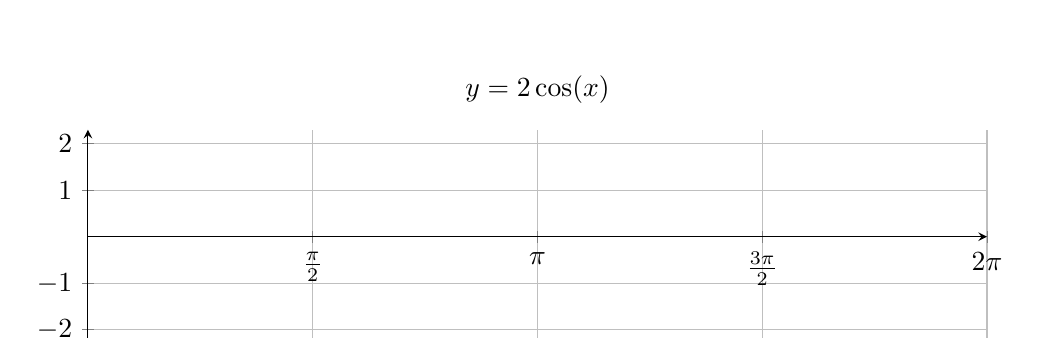
\begin{tikzpicture}
\begin{axis}[
    width=13cm,height=4.3cm,
    axis lines=middle,
    xmin=0,xmax=2*pi,ymin=-2.3,ymax=2.3,
    xtick={pi/2,pi,3*pi/2,2*pi},
    xticklabels={$ \frac{\pi}{2}$,$\pi$,$\frac{3\pi}{2}$,$2\pi$},
    ytick={-2,-1,1,2},
    grid=major,
    title={$y=2\cos(x)$}
]
\end{axis}
\end{tikzpicture}

\vspace{0.5cm}

\begin{tikzpicture}
\begin{axis}[
    width=13cm,height=4.3cm,
    axis lines=middle,
    xmin=0,xmax=2*pi,ymin=-1.3,ymax=1.3,
    xtick={pi/2,pi,3*pi/2,2*pi},
    xticklabels={$ \frac{\pi}{2}$,$\pi$,$\frac{3\pi}{2}$,$2\pi$},
    ytick={-1,1},
    grid=major,
    title={$y=\sin\left(x+\frac{\pi}{2}\right)$}
]
\end{axis}
\end{tikzpicture}
\end{center}

\subsection*{Exercise 17: True or false?}
Tick the correct box. Correct every false statement.

\begin{center}
\renewcommand{\arraystretch}{1.6}
\begin{tabular}{p{10.8cm}|c|c}
\toprule
Statement & True & False\\
\midrule
The sine function has period $2\pi$. & $\square$ & $\square$\\
The cosine function starts at $0$. & $\square$ & $\square$\\
The maximum value of $3\sin(x)$ is $3$. & $\square$ & $\square$\\
The function $\sin(2x)$ has amplitude $2$. & $\square$ & $\square$\\
Sine and cosine have the same shape but are shifted horizontally. & $\square$ & $\square$\\
\bottomrule
\end{tabular}
\end{center}

\textbf{Corrections:}

\vspace{2cm}
\hrulefill

\newpage

% ============================================================
% PAGE 6 -- CHALLENGE
% ============================================================

\section*{Challenge: Describe a transformed sine function}

Consider
\[
f(x)=3\sin\left(\frac{x}{2}-\pi\right)+1.
\]

Without drawing the graph, determine:

\begin{tabular}{p{0.45\textwidth}p{0.45\textwidth}}
Amplitude: \answerline[5cm] &
Period: \answerline[5cm] \\[1.2cm]
Horizontal shift: \answerline[5cm] &
Vertical shift: \answerline[5cm]
\end{tabular}

Explain in one or two sentences how the graph differs from $y=\sin(x)$.

\vspace{2cm}
\hrulefill

\vspace{2cm}
\hrulefill

\vfill

\emph{Remember: sine and cosine are not only triangle ratios. Their graphs are
the basic mathematical shapes of oscillations and waves.}

\newpage

% ============================================================
% PAGE 7 -- EXERCISES 6--9
% ============================================================

\section*{Exercise 6}
Determine the period of the following functions and arrange them from the
shortest period to the longest period.

\begin{enumerate}[label=\alph*)]
\item $y=\sin(x)+4$
\item $y=\sin\left(2x+\frac{\pi}{2}\right)+1$
\item $y=\sin(3x)$
\item $y=\sin\left(\frac34x\right)$
\item $y=\cos(4x-1)-2$
\item $y=\cos\left(\frac14x\right)$
\end{enumerate}

\section*{Exercise 7}
Describe what happens in the following cases:
\begin{itemize}
\item The graph changes from $y=\cos(x)$ to $y=\cos(2x)+2$.
\item The graph changes from $y=\cos(x)$ to $y=\cos(0.5x)-3$.
\item The graph changes from $y=\sin(x)$ to $y=\sin(x-\pi)$.
\item The graph changes from $y=\cos(x)$ to $y=\cos\left(x+\frac{\pi}{2}\right)$.
\end{itemize}

\section*{Exercise 8}
Choose the correct function.

\begin{enumerate}
\item The graph has amplitude $1$ and period $\pi$:
\begin{multicols}{2}
\begin{itemize}[label=$\square$]
\item $\sin(x)$
\item $\sin(0.5x)$
\item $\sin(2x)$
\item $\sin(3x)$
\end{itemize}
\end{multicols}

\item The graph has amplitude $1$ and period $4\pi$:
\begin{multicols}{2}
\begin{itemize}[label=$\square$]
\item $\cos(x)$
\item $\cos(0.5x)$
\item $\cos(2x)$
\item $\cos(3x)$
\end{itemize}
\end{multicols}

\item Which function is shifted to the right by $\pi$ compared to $\sin(x)$?
\begin{multicols}{2}
\begin{itemize}[label=$\square$]
\item $\sin(x+\pi)$
\item $\sin(x-\pi)$
\item $\sin(2x)$
\item $\cos(x)$
\end{itemize}
\end{multicols}

\item Which function has the shortest period?
\begin{multicols}{2}
\begin{itemize}[label=$\square$]
\item $\sin(x)$
\item $\sin(2x)$
\item $\sin(5x)$
\item $\sin(0.25x)$
\end{itemize}
\end{multicols}
\end{enumerate}

\section*{Exercise 9}
Complete the functions --- fill in the missing numbers.

\begin{enumerate}
\item The period should become $\pi$:
\[
y=\sin(\blank{1.5cm}x)
\]

\item The period should become $4\pi$:
\[
y=\sin(\blank{1.5cm}x)
\]

\item The period should become $\dfrac{\pi}{2}$:
\[
y=\sin(\blank{1.5cm}x)
\]

\item The graph should be shifted to the right by $\pi$:
\[
y=\sin(x\mathbin{\pm}\blank{1.5cm})
\]

\item The graph should be shifted to the left by $\dfrac{\pi}{2}$:
\[
y=\cos(x\mathbin{\pm}\blank{1.5cm})
\]
\end{enumerate}

\newpage

% ============================================================
% PAGE 8 -- MODELLING REAL SITUATIONS
% ============================================================

\section*{Modelling Real Situations}

\subsection*{1. Two swinging pendulums}

Two pendulums swing with the same amplitude (\SI{1}{cm}).

\begin{itemize}
\item Pendulum A completes one full swing every $4$ seconds.
\item Pendulum B completes one full swing every $2$ seconds.
\item Both start at their highest position at $t=0$.
\end{itemize}

\begin{enumerate}[label=\alph*)]
\item Write down a cosine function for each pendulum.
\item Which pendulum has the longer period?
\item Which pendulum moves faster?
\item Which graph is stretched more along the time axis?
\end{enumerate}

\textit{Hint: It might be helpful to sketch the graphs.}

\vspace{1cm}

\subsection*{2. Build your own oscillation}

Your oscillation should have:
\begin{itemize}
\item amplitude $1$,
\item period $\pi$,
\item shifted by $\frac{\pi}{2}$ to the right.
\end{itemize}

Write a possible sine function describing this wave.

\vspace{1cm}
\[
\answerline[12cm]
\]

Is there another possibility to express the function, e.g.\ as a cosine
function?

\vspace{1cm}
\[
\answerline[12cm]
\]

\end{document}
